
\section{next steps}

\subsection{practicalities}

\begin{frame}[fragile]
\frametitle{technical skills for numerical ice sheet modeling}

\begin{itemize}
\item comfort in a technical computing environment; need to know:
  \begin{itemize}\small
  \item[$\circ$] an editor,
  \item[$\circ$] a scripting/prototyping language (Matlab, Python, etc.),
  \item[$\circ$] a compiled language (C or Fortran),
  \item[$\circ$] \emph{a version control system} (Subversion, git, etc.), and
  \item[$\circ$] some tools for NetCDF files
  \normalsize
  \end{itemize}
\item willingness to read math, numerical analysis, computer science, etc.
\item \emph{physics}
\end{itemize}
\end{frame}


\begin{frame}
\frametitle{technical skills for numerical ice sheet modeling 2}

\begin{itemize}
\item \emph{never} re-invent the wheel for basic numerics like these:
  \begin{itemize}
  \item[$\circ$] numerical linear algebra
  \item[$\circ$] mesh generation, finite element assembly and solve
  \item[$\circ$] \dots \emph{except} to write throw-away codes to help you understand numerical ideas 
  \end{itemize}
\item try existing ice flow models:
  \begin{itemize}
  \item[$\circ$] open source SIA-based comprehensive models: GLIMMER, SICOPOLIS
  \item[$\circ$] open source hybrid/higher-order/Stokes models: PISM, Elmer, ISSM
  \end{itemize}
\item ice sheet modeling is young, and much to do!
\end{itemize}
\end{frame}


\subsection{some omitted models}

\begin{frame}{thermomechanical coupling}

\begin{columns}
\begin{column}{0.5\textwidth}
\begin{itemize}
\item ice softness $A(T)$ varies by $10^3$ in relevant temperature range
\end{itemize}
\end{column}
\begin{column}{0.5\textwidth}
  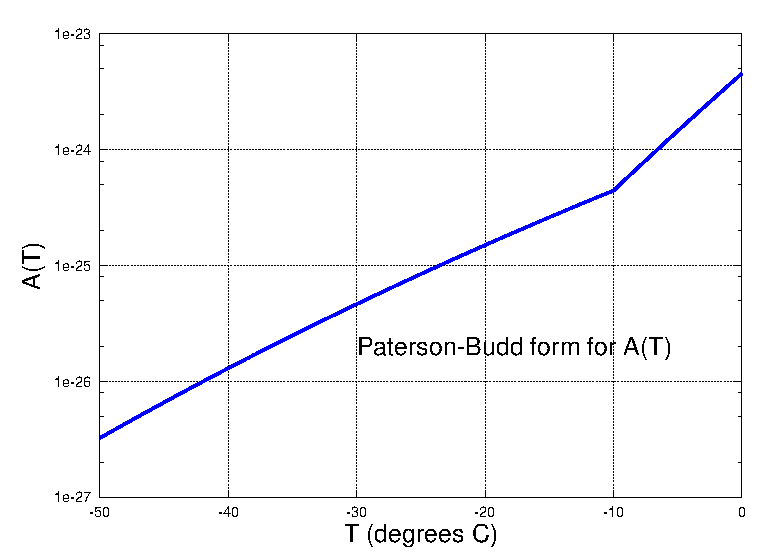
\includegraphics[width=1.0\textwidth]{AofT}
\end{column}
\end{columns}

\begin{itemize}
\item ice thermal state (temperature) gives ice sheet flows their ``long memory'' of past climate
\item dissipation of gravitational potential energy is major part of basal melt
  \begin{itemize}
  \item[$\circ$] each year, Jakobshavn drainage basin in Greenland dissipates enough gravitational potential energy to melt $> 1\,\text{km}^3$ of ice
  \item[$\circ$] geothermal flux also significant in slow parts
  \end{itemize}
\item so good ice sheet models need conservation of energy
  \begin{itemize}
  \item[$\circ$] ``enthalpy'' is good way to track energy content polythermally (Aschwanden et al.~2012)\nocite{AschwandenBuelerKhroulevBlatter}
  \end{itemize}
\end{itemize}

\end{frame}


\begin{frame}{solid Earth deformation}

\begin{itemize}
\item ice density is about $\frac{1}{3}$ that of rock in the Earth's mantle,
  \begin{itemize}
  \item[$\circ$] 1000 m of ice depresses the Earth's crust about 300 m
  \item[$\circ$] \dots if allowed enough time
  \item[$\circ$] how much time is determined by \emph{upper mantle viscosity}
  \item[$\circ$] \dots which is not perfectly known
  \end{itemize}
\item Earth deformation changes bed topography and thus ice flow
\item modeling Earth deformation is most important to modeling ice flow over long time scales (Peltier, 1998)\nocite{Peltier1998review}
\end{itemize}

\begin{center}
  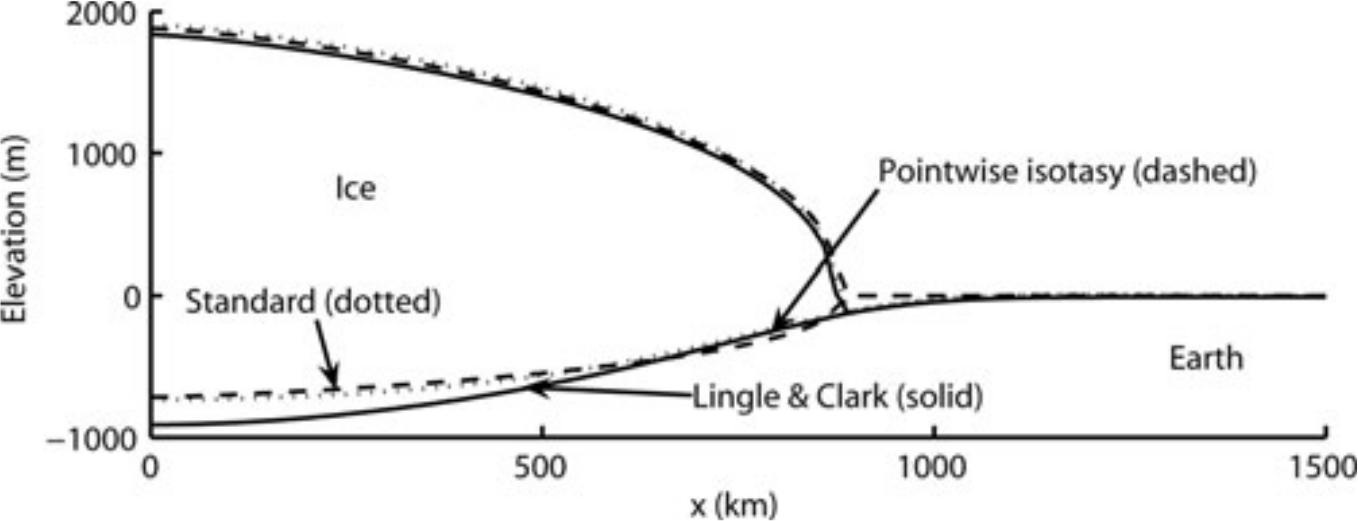
\includegraphics[width=0.75\textwidth]{earthcompare}
\end{center}
\end{frame}


\begin{frame}{spin-up}

\begin{itemize}
\item direct observations are not enough to initialize an ice sheet flow model
  \begin{itemize}
  \item[$\circ$] because ice temperature is a ``hidden variable'', and
  \item[$\circ$] because sliding depends on additional liquid water ``hidden variables'' at base
  \end{itemize}
\item two options exist to initialize:
  \small
  \begin{enumerate}
  \item \emph{traditional choice}: use low-dimensional time series data from physical surrogates (e.g. $\delta \phantom{|}^{18}O$ record from ice cores) for paleoclimate record; hope a long model run ends with a good current state
  \item \emph{promising alternative}:  use rich and spatially-distributed mostly-surface observations of present ice sheet state to reconstruct initial state using ``inversion'' of PDEs
  \normalsize
  \end{enumerate}
\end{itemize}
\end{frame}


\begin{frame}{inverse modeling}

\begin{itemize}
\item stress balance PDEs can turn extra boundary data on top into missing basal information
\item surface velocity observations can be inverted to find basal shear stress (below)
\item mostly future: invert radar layers (isochrones)
\end{itemize}

\begin{center}
  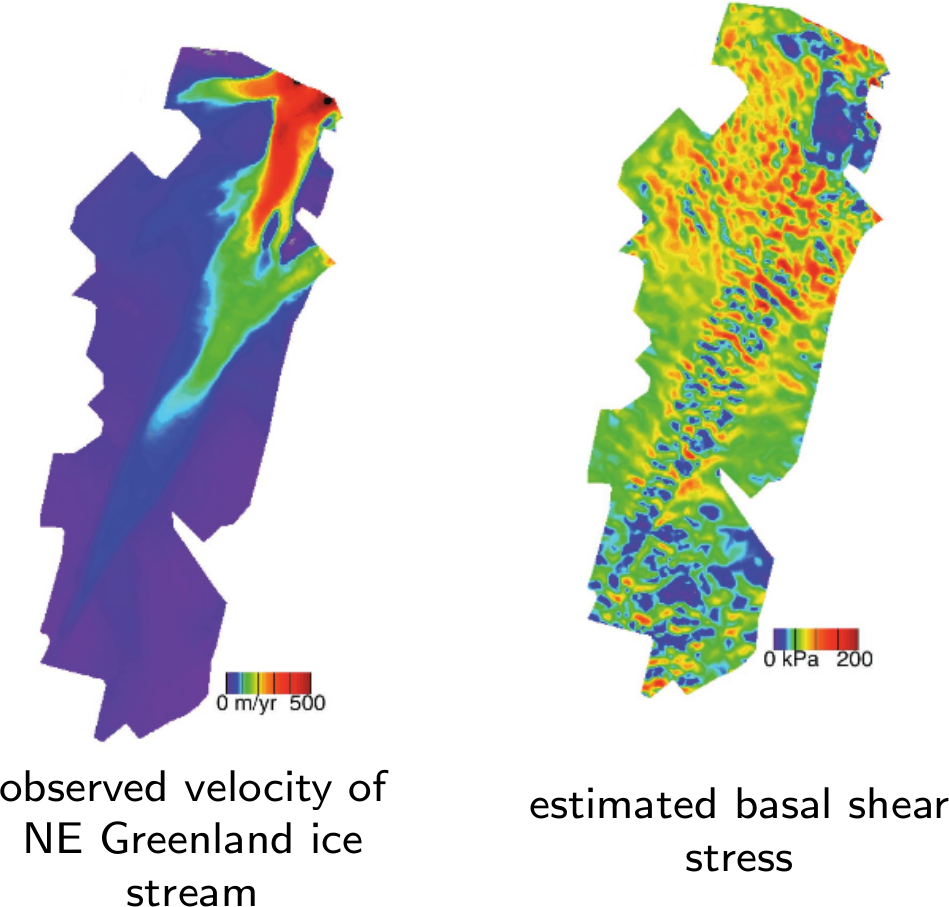
\includegraphics[width=0.6\textwidth]{NEgreenlandJoughin}
  
  \medskip
  \tiny from Joughin et al.~(2001)\nocite{Joughinetal2001}
\end{center}
\end{frame}


\begin{frame}{Stokes equations and solvers}

\begin{itemize}
\item the Stokes model itself, without shallow assumptions, can be solved numerically, \alert{but}:
  \begin{itemize}
  \item[$\circ$] many equations in many unknowns, especially in 3D
  \item[$\circ$] requires explicit accounting for incompressibility---a constraint on the flow---through a pressure variable
  \item[$\circ$] ice sheets are \emph{actually} shallow, and the aspect ratio of grid elements can be a problem
  \end{itemize}
\item much of the success so far is at a smaller scale
\end{itemize}

\begin{columns}
\begin{column}{0.45\textwidth}
\scriptsize

Figure 7 in Maxwell et al.~(2008)\nocite{Maxwelletal2008}:  velocity contour lines ($\text{m}\,\text{a}^{-1}$) for Athabasca Glacier from \textbf{a} Stokes model, \textbf{b} measurements (Raymond, 1971)\nocite{Raymond1971}
\end{column}
\begin{column}{0.6\textwidth}
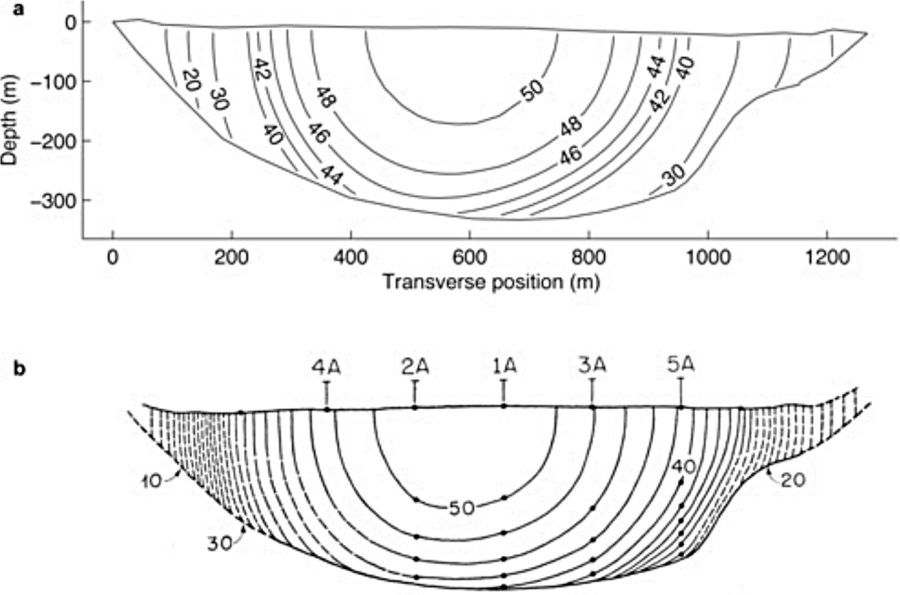
\includegraphics[width=1.0\textwidth]{athabasca}
\end{column}
\end{columns}
\end{frame}


\begin{frame}{``higher-order'' schemes}

\begin{itemize}
\item both the SIA and the SSA are derived by small-parameter arguments from the Stokes equations, so \dots is there a \emph{common shallow antecedent model}?
\item Schoof and Hindmarsh (2009)\nocite{SchoofHindmarsh} answer:  \emph{yes}, the model derived by Blatter (1995)\nocite{Blatter} is an intermediate model
\item a hierarchy:
\end{itemize}
\begin{center}
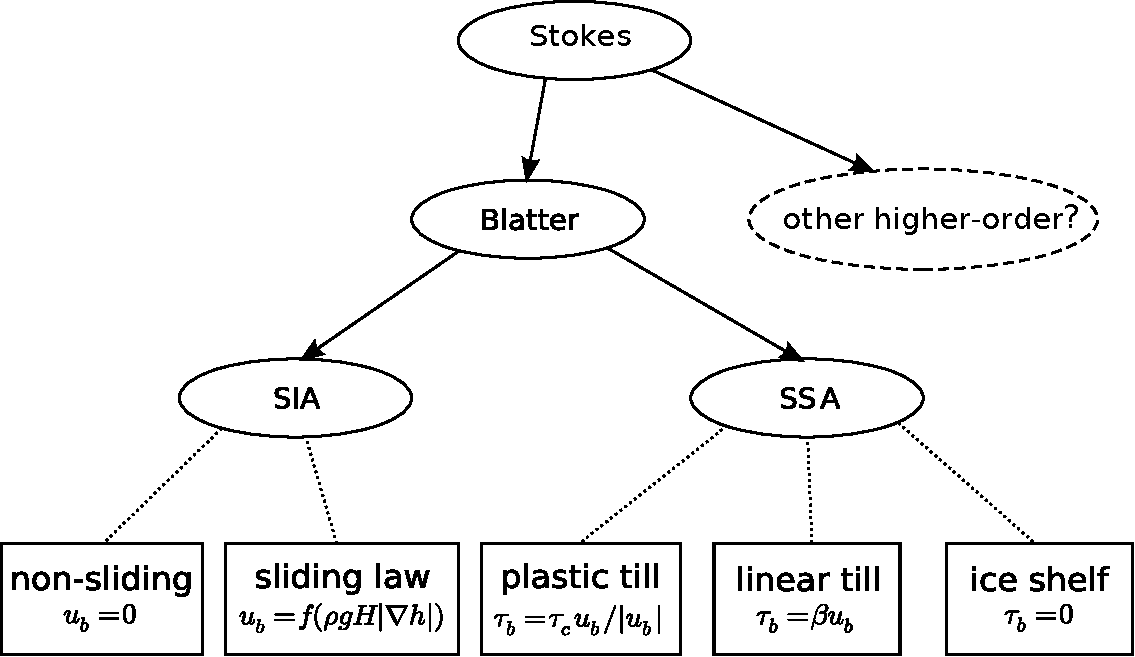
\includegraphics[width=0.8\textwidth]{hierarchy}
\end{center}
\end{frame}


\begin{frame}{shallow hybrid schemes}

\begin{itemize}
\item so how about ``gluing together'' SIA and SSA?
\item there are multiple schemes for hybridization (Pollard and deConto, 2007\nocite{PollardDeConto}; Bueler and Brown, 2009\nocite{BBssasliding}; Goldberg 2011\nocite{Goldberg2011})
\item shallow hybrids can be used \emph{now} at high spatial resolution and paleoglacial time scales
\item for example, we can compare observed (left) and 1km grid modeled (middle and right; model=PISM) surface velocity maps for the Greenland ice sheet
\end{itemize}

\vspace{-4mm}
\begin{center}
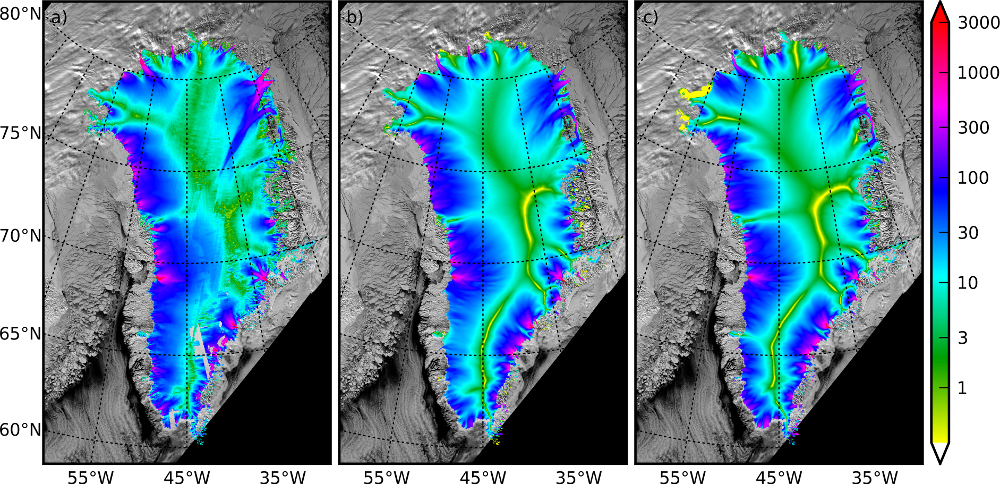
\includegraphics[width=0.9\textwidth]{csurf_insar_pism_1km}
\end{center}
\end{frame}
